\documentclass[11pt]{article}
\usepackage{classTools}

\begin{document}

% To include a problems set header, use the psHeader command
\psHeader{4}{Wed Oct. 9, 2024 (11:59pm)}

\textbf{Your name: Roshen Chatwal}

\textbf{Collaborators: Aidan Pesce, Raunak Daga }

\textbf{No. of late days used on previous psets: 24 minutes}

\textbf{No. of late days used after including this pset: Probably 1 by now }

\begin{enumerate}
    \item (Randomized Algorithms in Practice)  
    \begin{enumerate}
        \item Implement Randomized QuickSelect, filling in the template we have given you in the Github repository.
        
        \item 
        In the repository, we have given you datasets $x_n$ of key-value pairs of varying sizes to experiment with: dataset $x_n$ is of size $n$.  For each dataset $x_n$ and any given number $k$, we will consider how to efficiently answer the $k$ selection queries
        $\select(x_n,0)$, $\select(x_n,[n/k])$, $\select(x_n,[2n/k])$, $\ldots$, $\select(x_n,[(k-1)n/k])$ on $x_n$, where $[\cdot]$ denotes rounding to the nearest integer. For example, if $k=4$, then we release the minimum, the 25th percentile, and the 75th percentile of the dataset.  You will compare the following two approaches to answering the queries:
        
        \begin{enumerate}
            \item Running (randomized) \QuickSelect{} $k$ times.
            \item Running \MergeSort{} (provided in the repository) once and using the sorted array to answer the $k$ queries.
        \end{enumerate}
        Specifically, you will compare the {\em distribution} of runtimes of the two approaches for a given pair $(n,k)$ by running each approach many times and creating density plots of the runtimes.  The runtimes will vary because \QuickSelect{}  is randomized, and because of variance in the execution environment (e.g. other processes that are running on your computer during each execution). \vspace{1.5mm}
        
        We have provided you with the code for plotting. Before plotting, you will need to implement \MergeSortSelect{}, which extends \MergeSort{} to answer $k$ queries. Your goal is to use these experiments and the resulting density plots to propose a value for $k$, denoted $k^*(n)$, at which you should switch over from \QuickSelect{} to \MergeSortSelect{} for each given value of $n$ (you can choose any reasonable statistical feature to propose $k^*(n)$, such as the peak runtime of the distribution or the mean runtime, etc). Do this by experimenting with the parameters for $k$ (code is included to generate the appropriate queries once the $k$'s are provided) and generate a plot for each experiment.  Explain the rationale behind your choices, and submit a few density plots for each value of $n$ to support your reasoning.  (There is not one right answer, and it may depend on your particular implementation of \QuickSelect{}.) \\
        
\textcolor{blue}{
I started off by looking at k values of 5, 10, 20, 30, 40 to broadly gauge how many select queries would be needed for the distribution of \QuickSelect{} runtimes to center around a slower time than the distribution of \MergeSortSelect{} runtimes. Relative horizontal positioning of the curves' peaks was my main measure because it gives an approximate number line location of the expected runtime of an algorithm. I noticed that the blue curve's peak seemed slight to the right of the orange curve's peak for k = 30 on N = 1024, so I increased RUNS to 50 for a more reliable capture of the runtime distribution and narrowed my range of experimental k-values between 27-31. The blue peak was just right of the orange peak when k=28, so I settled on $k^*(1024)=28$. Moving down a row, I noticed that the blue curve's peak seemed slight to the right of the orange curve's peak for k = 29 on N = 2048, so I settled on $k^*(2048)=29$. Repeating this process of experimental value range expansion and eyeballing peaks of the \QuickSelect{} runtime distribution closest to the right of the peaks of the \MergeSortSelect{}{} runtime distribution, I ended up with the following graphs with $k = k^*(n)$ for each of the provided input sizes:
}

\begin{figure}[H]
    \centering
    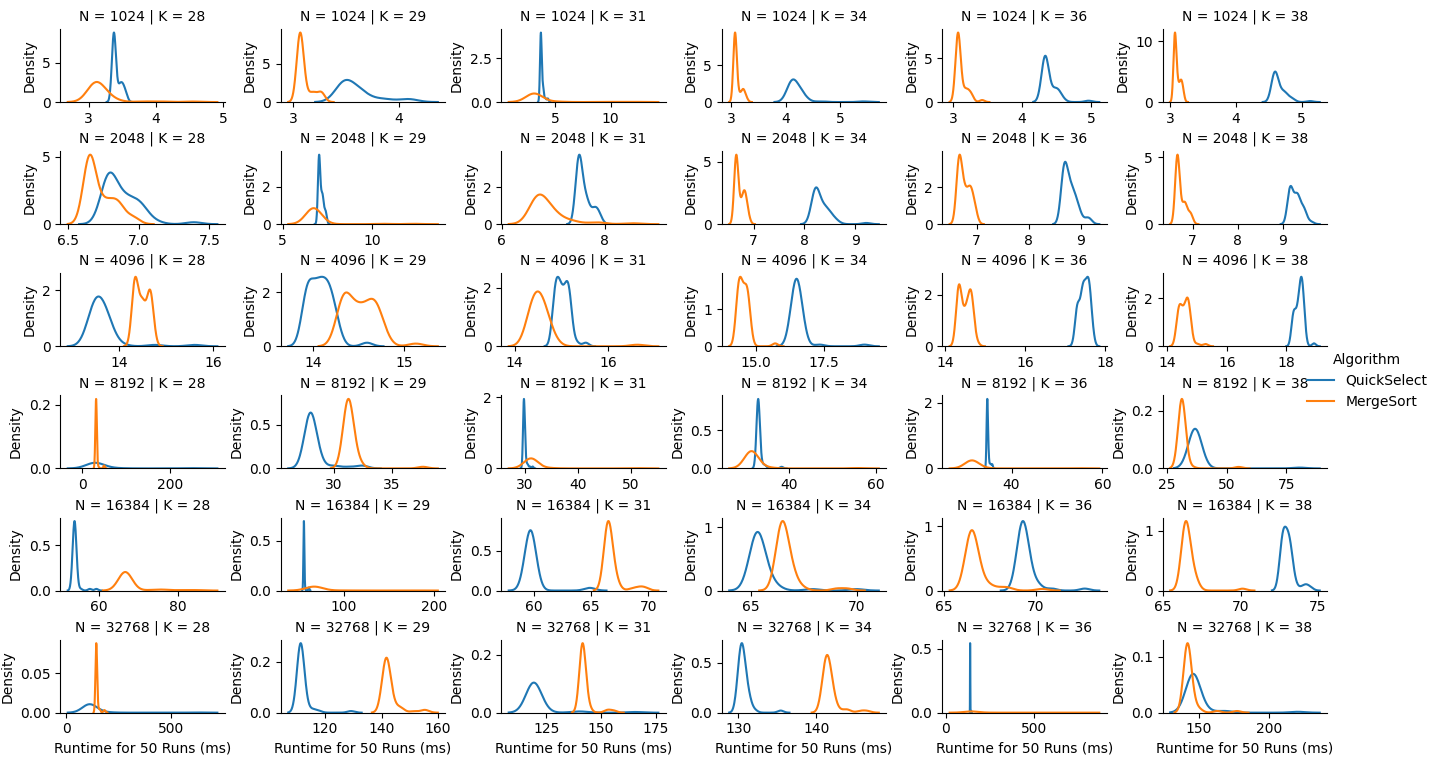
\includegraphics[width=1.1\linewidth]{PS4-1b.png}
    \caption{$k^*$ for each of the 6 input sizes provided and runtime graphs}
\end{figure}

\textcolor{blue}{
Below is a table that summarizes my interpreted $k^*$ values seen above. Notice how in the graphs above, the blue peak is just to the right of the orange peak along the main diagonal of graphs from top left to bottom right. These graphs, relative to other experimental graphs, are what informed my discretion when identifying $k^*$. 
}\\

\textcolor{blue}{
\begin{tabular}{| c | c |}
\hline
n       & $k^*(n)$       \\ \hline
1024   & 28   \\ \hline
2048   & 29  \\ \hline
4096   & 31   \\ \hline
8192   & 34  \\ \hline
16384   & 36  \\ \hline
32768   & 38  \\ \hline
\end{tabular}
} \\
        
        \item Extrapolate to come up with a simple functional form for $k^*(n)$, e.g. something like $k^*(n)=3\sqrt{n}+6$ or $k^*(n)=10\log^2 n$. (Again there is not one right answer.)  Briefly discuss how your extrapolation aligns with theoretical values. That is, what kind of functional form for $k^*(n)$ (in asymptotic notation) would be predicted by  the asymptotic runtimes of \QuickSelect{} and \MergeSortSelect{} for answering $k$ selection queries on a dataset of size $n$? \\

\textcolor{blue}{
        I noticed in my table that subsequent n values were double the previous (and powers of two). The $k^*$ values seemed to be incrementing by roughly the same amount (+1–3) as I moved down the rows. Intuitively, I gathered that we could treat the n values as an axis on a log-scale and the $k*(n)$ values as an axis on an ordinary scale, leading to a graph that looks linear. From this, I extrapolated the existence of an approximately logarithmic relationship between $k^*$ and $n$, which would at its most basic have functional form $k^*(n) = a\log_2{n} + c$ (it's 
        $\log_2$ because the input sizes double for subsequent runnings of the algorithms).} \\

\textcolor{blue}{
        To get approximations for $a$ and $c$, I entered my table into the Desmos online calculator and got it to find those coefficients for a logarithmic regression with base two.} \\
    

        \begin{figure}[H]
            \centering
            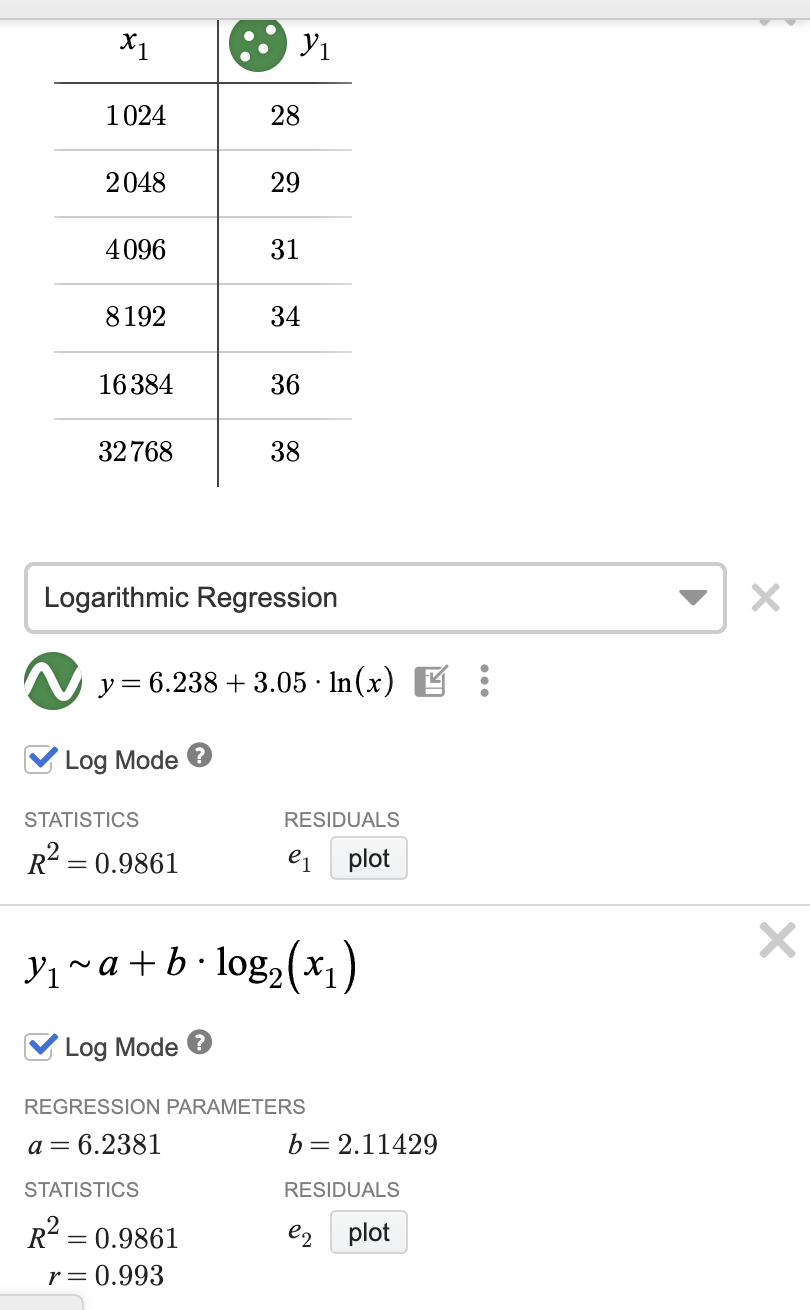
\includegraphics[width=0.25\linewidth]{DesmosReg.png}
            \caption{Desmos regression for coefficients}
            \label{fig:enter-label}
        \end{figure}

\textcolor{blue}{
        Using this information, my simple functional form for $k^*$ is $k^*(n) = 6.2\log_2{n} + 2.1$.} \\
        
\textcolor{blue}{
        This extrapolation aligns well with the theoretical values, as $k^*$ asymptotically scales in $O(\log{n})$ (base 2 is implied). When setting up the asymptotic runtimes of k queries of \QuickSelect{} and \MergeSortSelect{} equal, we get the equation $O(k^*n) = O(k^*n\log{n})$. This equality implies that k grows logarithmically with n to balance the extra logarithmic term in the worst case runtime for \MergeSortSelect{}. For further intuition on that, notice how the $k^*n = k^*n\log{n}$ identity only holds true when $k=0$ (trivial case) or $\log{n} = 1$. The latter case hints $k^*$ must grow proportionally to $\log{n}$ to prevent the \MergeSortSelect{} runtime from growing significantly faster than the \QuickSelect{} runtime. Therefore, theoretical $k^*$ scales in $O(\log{n})$, which is also true for my extrapolation of $k^*$ asymptotically.} \\

        
        \item (*optional)  One way to improve \QuickSelect{} is to choose a pivot more carefully than by picking a uniformly random element from the array. A possible approach is to use the \textit{\textbf{median-of-3}} method: choose the pivot as the median of a set of 3 elements randomly selected from the array. Add \MedianQuickSelect{} to the experimental comparisons you performed above and interpret the results.  That is, in what way (if any) does \MedianQuickSelect{} offer benefits over \QuickSelect{}?        \\

        \textcolor{blue}{
        I modified the function for \QuickSelect{} to choose three random, unique indices instead of one and let the pivot equal the median key out of the three quantities $arr[p_i][0]$ for $1 \leq i \leq 3$. Then, I made sure to run tests on \MedianQuickSelect{} and graph the the runtime distributions of \QuickSelect{}, \MedianQuickSelect{}, and \MergeSortSelect{} using my original $k^*$ values from part (b) to enable as much of an apples-to-apples runtime comparison as possible. Below is what it looked like:
        }

        \begin{figure}[H]
            \centering
            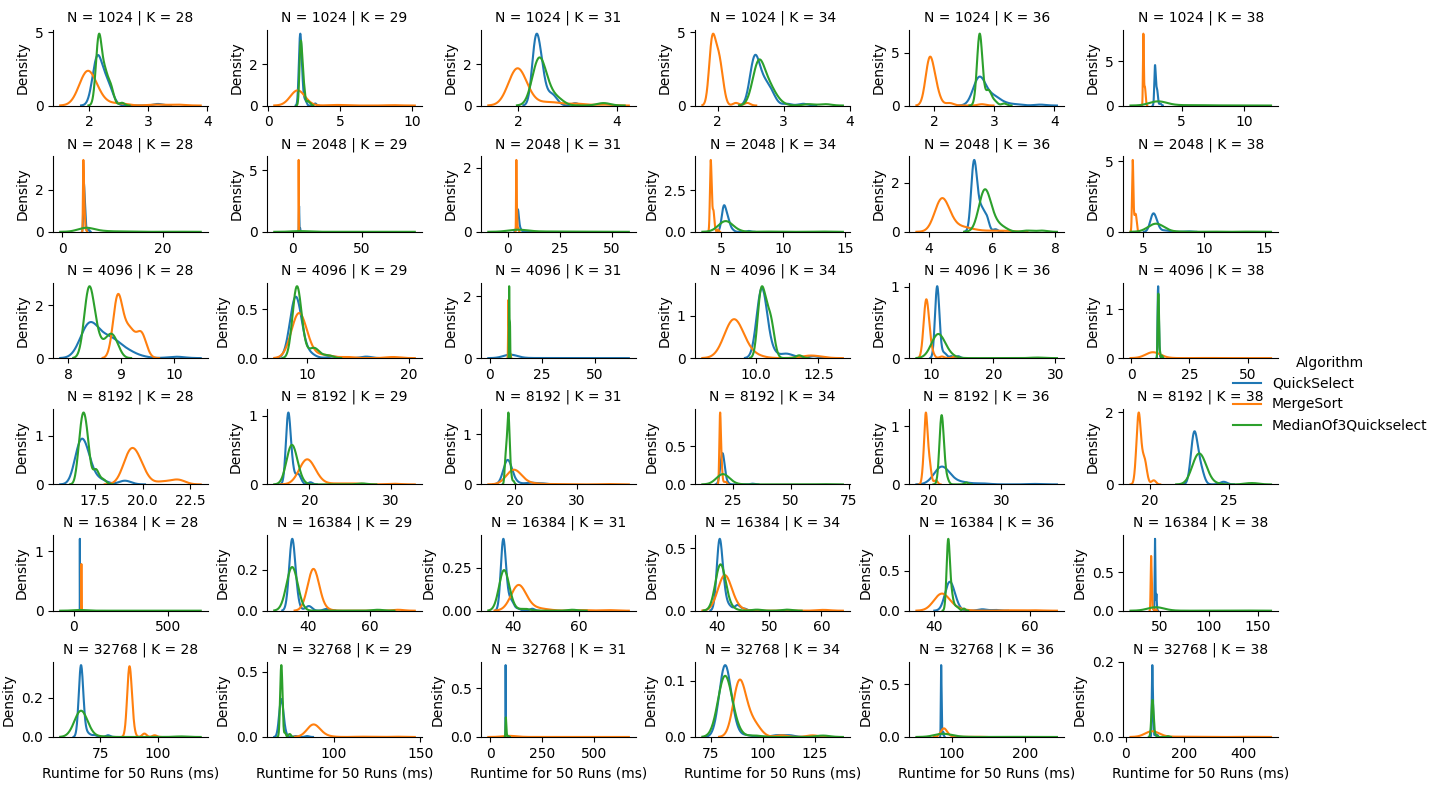
\includegraphics[width=1.1\linewidth]{medof3.png}
            \caption{New Runtime Distribution Comparison w/ \MedianQuickSelect{} }
            \label{fig:enter-label}
        \end{figure} \\

         \textcolor{blue}{
        As seen in the graphs above, the green curve most often centers exactly where the blue curve does. The variance of the \MedianQuickSelect{} runtime distribution tends to appear as greater than the variance of \QuickSelect{} (green curve is often more spread out), but I can't tell whether there's a significant difference. Thus, it's hard to conclude whether my implementation of \MedianQuickSelect{} in reality offers efficiency benefits over \QuickSelect{} over many queries. This would be because the expected runtime of \QuickSelect{} over many queries would be the average of runtimes when unlucky, lucky, and mediocre pivots are chosen (which should be near the expected runtime of \MedianQuickSelect{} which picks mediocre pivots with higher frequency by taking medians). I would expect that \MedianQuickSelect{} may be more helpful when there's a low number of queries and we are in a loss aversion mentality (i.e., even though \QuickSelect{} and \MedianQuickSelect{} asymptotically have the same worst-case runtimes, we'd prefer getting mediocre pivots consistently rather than a mix of unlucky and lucky pivots because we \textit{really} don't like the unlucky ones.
        } \\

        
        
    \end{enumerate}


    \item (Dictionaries and Hash Tables) 
    Consider the following computational problem:
    
\compprob{DuplicateSearch()}
{An array $(a_0,\ldots,a_{n-1})$ of natural numbers (each fitting in one word).}
{A duplicate element; that is, a number $a$ such that there exist $i \neq j$ such that $a_i = a_j = a$.}
\begin{enumerate}
    \item Show that DuplicateSearch can be solved by a Las Vegas algorithm with expected runtime $O(n)$ using a dictionary data structure.  (You should prove correctness and analyze runtime quoting the expected runtimes stated for the Dictionary data structure in Lecture 9, but you do not need to do a formal probability calculation using expectations.)  \\

    \textcolor{blue}{
        \textbf{Randomization (Viva Las Vegas!)}:
        The randomization in this algorithm comes from the picking of our random hash function $h_{\ell}$, where $h_{\ell}: [U] \rightarrow [m]$, where $\ell \in [R]$ for some number R. Note that once we know our specific $h_{\ell}$, there's nothing random left about the function. In this Las Vegas algorithm, we can allow $R = 1$, thus only leaving us with the choice of $h_0$ (although we're still "randomly" assigning $\ell = 0$ from the elements of $[R]$). Let $h_0(K) = K \mod m$. This hash function will map every natural number in our input array to a value $x : x \in [m]$. Of course, R could be larger and we could have R correct hash functions mapping values from $[U] \rightarrow [m]$, but I'm setting R=1 for this example because it makes life easy (and because I can since R is "some number").
    } \\
    
    \textcolor{blue}{
        \textbf{Preprocessing}:
        Initialize a hash table H of size $m$, where $0 \leq m \leq n$. Let's simply let $m = \lfloor \frac{n}{2} \rfloor$ (we'll see how this is useful later). The hash table is a variant of a dynamic dictionary data structure. Our initialized H will have elements' keys equalling their dictionary index locations and elements' values being empty linked lists (which will later be populated with the input array's natural numbers $a_i$ where $h_{\ell}(a_i)$ equals the key).
    } \\

\textcolor{blue}{
\textbf{DuplicateSearch Process:}
\begin{itemize}
    \item For \( i \) in range(\( n \)):
    \begin{itemize}
        \item Traverse the input array and compute \( h_{\ell}(a_i) \)
        \item GOTO \( [h_{\ell}(a_i)][1] \)
        \item Search if \( a_i \) is already in the linked list
        \item If so:
        \begin{itemize}
            \item Return \( a_i \)
        \end{itemize}
        \item If not:
        \begin{itemize}
            \item Append \( a_i \) to the linked list at \( [h_{\ell}(a_i)][1] \), making it the new head
        \end{itemize}
    \end{itemize}
    \item Return $\bot$ \\
\end{itemize}
} 

\textcolor{blue}{
\textbf{Correctness}:
        This algorithm is correct because when we're at the $i^{th}$ element of the input array and find that $a_i$ already exists in the hash table through a search, we know that we must've seen an $a_j$ such that $a_j = a_i$ at a previous index of our input array. Thus, we know that $a_i$ is a duplicate element, and by returning $a_i$, we are returning a duplicate element. In the case where there's no duplicate elements in the array, we'll only return $\bot$ because it's the default value we return when no $a_i$ we iterate over is found in the linked list its duplicate would've been located in. Since the algorithm is both always correct, as proven through my statements above, and using randomness, I have proven that DuplicateSearch can be solved by a Las Vegas algorithm.
    } \\

\textcolor{blue}{
    \textbf{Runtime Analysis}: \\
    Let's break down the expected runtime of this Las Vegas algorithm in terms of the worst-case and expected worst-case runtimes of its steps:
    \begin{enumerate}
        \item Picking our random hash function takes a constant number of steps, taking $O(1)$ time.
        \item Initializing our hash table H takes $O(m)$ time, as we need to initialize $m$ $(K,V)$ pairs with $K$ being the pair's index location in H and $V$ being an empty linked list. Note that $m = \lfloor \frac{n}{2} \rfloor$, so by eliminating floor notation for simplicity, this step takes $O(\frac{n}{2})$ time.
        \item The maximum expected time it takes to iterate over each $a_i$ until returning some outcome is $n \cdot O(T_{\text{compute-hash}} + E[T_{\text{search-linked-list}}] + T_{\text{append-list}}) + O(T_{\text{return-bot}}) = n \cdot(O(1) + O(3) + O(1)) + O(1) = n \cdot(O(1) + O(1) + O(1)) + O(1) = n \cdot O(1) + O(1) = O(n+1) = O(n)$ time.
        \begin{enumerate}
            \item By the \textit{efficient evaluation property} of random hash functions, $T_{\text{compute-hash}}(a_i)$ takes $O(1)$ time.
            \item The reason we use expected time for search is because we expect a linked list to have, on average, $\frac{n}{m}$ elements due to the \textit{low chances of collision} property of random hash functions. So even though a list could theoretically contain all $n$ input elements if we're unlucky, we use the expected length of the linked list to reflect the linked list length that's most likely on average. Expected search time thus takes $O(1 + \frac{n}{m})$ time since we have to take a step jumping to the correct linked list and, on average, search through $\frac{n}{m}$ linked list elements that don't match $a_i$. Keep in mind our (simplified) definition of $m = \frac{n}{2}$, which thus makes this step equivalently take $O(1 + \frac{n}{\frac{n}{2}}) = O(1+2) = O(3) = O(1)$ time, asymptotically.
            \item $T_{\text{append-list}}$ requires one step (since only the head of the linked list is manipulated) and thus takes $O(1)$ time.
            \item In the worst case, we will have looped through the processes mentioned in (i-iii) $n$ times and never have returned a duplicate (meaning all $n$ of our natural number inputs have been inserted in the linked lists in H). Since we're sure there's no duplicates by this point, we return $\bot$ and this takes $O(1)$ time.
        \end{enumerate}
    \end{enumerate}
    Aggregate Runtime: Combining the times for Randomization, Preprocessing, and DuplicateSearching, we get that our Las Vegas algorithm takes $O(1) + O(\frac{n}{2}) + O(n) = O(n)$ expected runtime asymptotically (this is entirely made possible because $m = \theta(n)$). This concludes our proof, as \textbf{I've shown that my correct Las Vegas algorithm has expected runtime in $O(n)$.}
} \\

    \item DuplicateSearch can be solved by a deterministic algorithm in runtime $O(n\log n)$. Briefly describe this algorithm in 2-3 sentences (you do not need to write a pseudocode and do not need to provide a proof of correctness). \\

\textcolor{blue}{
As opposed to a Las Vegas algorithm, this deterministic algorithm has a fixed execution path and uses no randomness. The $O(n\log n)$ runtime seems awfully suggestive of \MergeSort{}, so I'll describe how DuplicateSearch can be reduced to sorting (and use \MergeSort{} as the oracle).
} \\

\textcolor{blue}{
    \textbf{Procedure:} \\
    \\
    No preprocessing needed. We run \MergeSort{} (the oracle) on our input array. Let's call the the sorted array A'. Then, for postprocessing, we iterate over $A'[i]$ and $A'[i+1]$ for all $i \in [n-1]$, checking whether any adjacent locations $A'[i]$ and $A'[i+1]$ contain equivalent natural numbers. Whenever we \textit{observe} that $A'[i] == A'[i+1]$ for some valid $i$, we simply return $A'[i]$ because that's a duplicate number in our input array as well as our sorted array. If we \textit{never observe} that $A'[i] == A'[i+1]$ for any valid $i$, we return $\bot$ because that means there were no duplicate natural numbers in our sorted or input arrays.
} \\

\textcolor{blue}{
    \textbf{Runtime Analysis:} \\
    \begin{enumerate}
        \item MergeSort takes $O(n\log{n})$ time.
        \item Each iteration over adjacent numbers in $A'$ takes a constant number of steps to check for equality between $A'[i]$ and $A'[i+1]$. When our input array has no duplicate natural numbers, we end up iterating through $n-1$ adjacent number pairs in $A'$. Thus, the loop takes $(n-1) \cdot O(1) = O(n-1) = O(n)$ time asymptotically.
        \item Returning $\bot$ after the loop fails to yield a duplicate natural number takes $O(1)$ time.
    \end{enumerate}
    \textbf{Aggregate Runtime}: Combining the asymptotic runtimes for \MergeSort{}, postprocessing, and returning $\bot$, we can see that the deterministic algorithm for solving DuplicateSearch takes $O(n\log{n}) + O(n) + O(1) = O(n\log{n})$ time asymptotically.
} \\

\end{enumerate}    
    

 \item (Choosing Algorithms and Data Structures)
     Suppose the US Census Bureau was going to develop a new database to keep track of the exact ages of the entire US population, and publish statistics on it.  The data it has on each person is an exact birthdate
    $\bday$ (year, month, and date) and a unique identifier $\id$ (e.g. social security number --- pretend that these are assigned at birth). 
    
    For each of the three scenarios below, 
    \begin{enumerate}
        \item Select the best algorithm or data structure for the Census Bureau to use from among the following: 
        \begin{itemize}
            \item sorting and storing the sorted dataset 
            \item storing in a binary search tree (balanced and possibly augmented)
            \item storing in a hash table
            \item running randomized QuickSelect. 
        \end{itemize}
        \item Explain how you would use the
        algorithm or data structure (including any necessary augmentations) to solve the stated problem, e.g. what would you take as keys and values, what updates and queries (in case you use a dynamic data structure) would you issue, and how you would read off the results to obtain the desired statistics. 
        \item State what the runtime would be as a function of all of the relevant parameters: the size $n$ of the US population being surveyed, the number $u$ of updates issued at the specified time intervals, and/or the number $s$ of statistics released at the specified time intervals.     (These parameters are not all freely varying in the parts below, e.g. $s$ may be a fixed constant or a function of $n$; state any such constraints in your answers.) 
    \end{enumerate}
    In each scenario, you should assume (unrealistically) that the described queries or statistics are the {\em only} way in which the data is going to be used, so there is no need to support anything else.
        
\begin{enumerate}
\item (Reporting Age Rankings)
Every ten years as part of the Decennial Census, the Bureau collects a fresh list of $(\id,\bday)$ pairs from the entire US population.
(It does not reuse data from the previous Decennial Census, so everyone is re-surveyed.)
In order to incentivize participation, the Bureau promises to tell every respondent their age-ranking in the population after the survey is done (e.g. ``you are the 796,421'th oldest person among those who responded to the Census'').

\item (Daily Quartiles)
After each day, the Bureau obtains a list of $(\id,\bday)$ pairs to add to or remove from its database due to births, deaths, and immigration, and publishes an updated 25th, 50th, and 75th percentile of the population ages.

\item (Age Lookups)
For privacy reasons, the Bureau decides to not publish any statistics on the population ages, but just wants to maintain a database where the age of any member of the population can be looked up quickly, and the database can be quickly updated daily according to births, deaths, and immigration. \\
 \end{enumerate}

\textcolor{blue}{
\textbf{Scenario 1: Reporting Age Rankings} \\ \\
\textbf{a.)} The best algorithm for the Census Bureau to use would be sorting and storing the stored dataset. This because we simply need to get our array of people in order from youngest to oldest, which can be done by sorting the array of $(K,V)$ pairs where the keys are a person's age and the values are a person's id. Once we have a sorted array, we simply tell each person they're the $(i+1)^{th}$ oldest person, where $i$ is the index of their $(K_i, V_i)$ data in the sorted array in order of age. \\ \\
\textbf{b.)} To reduce ReportingAgeRankings to Sorting, I'll need to preprocess the freshly collected list of people's $(id, bday)$ pairs into something that we can sort on. I'll simply do this by iterating over each $(id, bday)$ pair in the list, converting each person's "bday" to their age in days, and appending the $(ageindays, id)$ to a list originally initialized as empty. Then, I'll run \MergeSort{} on the array of $(ageindays, id)$, treating the quantity of $ageindays$ as the keys, to get a sorted array.\\
There's no updates to worry about in this scenario since the list of $(id, bday)$ pairs collected is static since it's not being changed (other than when it's replaced as the default list after every Decennial Census) \\
Finally, for postprocessing/returning individual statistics, I'll just traverse over each of the $n$ respondents in the sorted array and tell them they're the $(i+1)^{th}$ oldest person in the US (where the index $i$ their data is located in the sorted array). \\ \\
I want to note that respondents with the same birthday in the same year will thus get different age-ranking depending on where their data was located in the original list, but that's a triviality I'll ignore since it probably doesn't really matter to the respondents whether they're ranked as older/younger than people born the same day as them. If I really wanted to, I could've handled ties by returning a ranking of the same $i+1$ for each person who has a duplicate birthday, where $i$ is the index of the first occurrence of the corresponding $ageindays$ in the sorted array.\\ \\
\textbf{c.)} Preprocessing takes $O(n)$ time since we're running a constant number of steps to calculate $ageindays$ for each person in the fresh list collected. Sorting takes $O(n\log{n})$ time when using \MergeSort{}. Returning age statistics to each repondents takes $O(n)$ time because it takes a constant number of steps to communicate to each of the $n$ respondents what ranking, $i+1$, they have in the sorted array by $ageindays$. There's no updates, as mentioned earlier. \\
Aggregating the analysis above, we get that $T_{ReportingAgeRankings}(n, u, s) = O(n + n\log{n} + s + 0u) = O(n\log{n} + s + 0u) = O(n\log{n} + s)$ asymptotically, where $s=n$ since this algorithm returns $n$ statistics (one for each respondent's age ranking).
} \\
\\

\textcolor{blue}{
\textbf{Scenario 2: Daily Quartiles} \\ \\
\textbf{a.)} The best data structure for the Census Bureau to use to quickly be able to access daily quartiles would be a balanced, size augmented BST. Balanced, size augmented BSTs are dynamic data structures that can relatively easily allow for the data to be updated (i.e. insertion or deletion of people's information from the database due to birth/immigration and debt can be done in $O(h) = O(\log{n})$ time in a balanced, size augmented BST per the solution of the DynamicDictionaries Problem seen in Lecture 5). Queries (i.e. selecting the $i^{th}$ largest key) also are relatively inexpensive in a size augmented, balanced BST and also take $O(h) = O(\log{n})$ time.  \\ \\
\textbf{b.)} To make the balanced, size augmented BST using our initial list of $(id, bday)$ pairs, I'd convert $bday$ to $ageindays$ like in Scenario 1 and then insert all $n$ people's $(ageindays, id)$ information as vertices in a balanced, size augmented BST called T. We use $ageindays$ as each vertex's key since people's relative ages are an important trait that need to be structured into the data structure being used to solve the Daily Quartiles problem. Every day that passes, we can simply increment every $ageindays$ up by 1 to reflect the passage of time. \\
Handling the daily updates (inserts/deletes) to T requires preprocessing the daily list of $(id, bday)$ pairs specified for insertion/removal from T into lists of $(ageindays, id)$ pairs. To update T, we simply insert the daily $(ageindays, id)$ pairs specified for insertion into T and delete the saily $(ageindays, id)$ pairs specified for deletion from T. \\
To publish each of the three quartiles daily, we just create variables representing the quantities $(\lceil T.size \cdot .25 \rceil)$, $(\lceil T.size \cdot .50 \rceil)$, and $(\lceil T.size \cdot .75 \rceil)$ for today's T. Then, we run a select query on T that will return us the the $i^{th}$ largest key in T (for $i$ values equal to the each of the three quantities defined above). These $i$ values intuitively correspond to the (indexes + 1) of a sorted list of $(ageindays, id)$ pairs in which we would find each desired quartile, as there's approximately $\frac{n}{4}$ keys between each quartile and the next (and approximately $\frac{n}{4}$ keys less than the $25^{th}$ percentile age and above the $75^{th}$ percentile age). \\ \\
\textbf{c.)} Preprocessing the initial list of $(id, bday)$ pairs takes $O(n)$ time like before and inserting each of the $n$ preprocessed pairs into our initial tree T takes $O(n\log{n})$ time (since insertion of one vertex into a size agumented, balanced BST takes $O(h) = O(\log{n})$ time and we must insert all $n$ vertices to get our initial T). The daily increment of every existing key value in T by 1 also takes $O(n)$ time. Our daily updates, insertion/deletion of vertices into T, each take $O(\log{n})$ time per our discussions in lecture 5. Returning our daily statistics, or the 25th, 50th, and 75th percentile of the population ages, take $O(log{n})$ time for each statistic as well per the size augmented, balanced BST properties discussed in lecture 5 (the size augmentedness of the tree enables this "$i^{th}$" key selection to run in $O(log{n})$ time). \\
Aggregating the the analysis above, we get that $T_{DailyQuartiles}(n, u, s) = O(n + n\log{n} + n + u(\log{n}) + s(\log{n})) = O(n\log{n} + u(\log{n}) + s(\log{n}))$ time asymptotically for $s=3$ on any given day since we're returning three quartile statistics.
} \\
\\

\textcolor{blue}{
\textbf{Scenario 3: Age Lookups} \\ \\
\textbf{a.)} Similar to problem 2, I would advise that the Census Bureau uses storing in a hash table to solve AgeLookups quickly while being able to quickly maintain the database to account for population changes. Since we don't need to publish any statistics dependent on the distribution of ages or order data by age, we can cut down the runtime of our database creation and maintainance and run quicker searches when the Bureau desires to look up someone's age. \\ \\
\textbf{b.)} For preprocessing, I would keep our initial list of $(id, bday)$ pairs. Then, I'd create an empty hash table H (a variant of a dynamic dictionary) of size $m$, where $m = \theta(n)$. Let's let $m = c\cdot n$, where $c \leq 1$, like we did in problem 2 for an easier runtime analysis later on. I would also pick a hash function that maps $[U] \rightarrow [m]$, and a simple one we could use is $h_{\ell}(n) = n \mod m$. $U$ in this case is the size of the $id$ universe. \\
To insert the data from our list of $(id, bday)$ pairs (an initial list or in an insertion update list due to births/immigration) into H, I'd evaluate $h_{\ell}(id')$ for each $(id', bday')$ in the list of $(id, bday)$ pairs. Then, I'd search the linked list at $H[h_{\ell}(id')]$ for $(id', bday')$. If it's not already there, I'll make $(id', bday')$ the new head of the linked list at $H[h_{\ell}(id')]$. If it's already there, I could do nothing or simply return a message saying that the person was already in H. For deletion of data from the hash table, I'd similarly evaluate $h_{\ell}(id')$ for each $(id', bday')$ in the deletion $(id, bday)$ pairs list and search the linked list at $H[h_{\ell}(id')]$ for $(id', bday')$. If it's not there, we don't do anything (or return $\bot$ or some warning note if we'd like an alert for attempting to delete some data that wasn't in H). If it's there, we simply remove $(id', bday')$ from the linked list at $H[h_{\ell}(id')]$. \\
To search for someone's birthday, assuming we know their unique $id$ number, we simply run $H[h_{\ell}(id)]$ and search the linked list at $H[h_{\ell}(id)]$ for an $(id, bday)$ where the $id$ equals the $id$ of the person whose birthday we want to look up. If such a pair exists, we extract $bday$ in that $(id, bday)$ pair and calculate $ageindays$. If a pair doesn't exist, we can return $\bot$ to signify that the $id$ we inputted in our search query was nowhere to be found in H (or some other error message). Our assumption that we can know a person's $id$ is why $id$ is the key in our $(id, bday)$ pairs and why we run $H[h_{\ell}]$ on the $id$, as it wouldn't make sense to be searching our hash table for a person's age if we already knew their birthday prior to searching H.\\ \\
\textbf{c.)} Our use of the original $(id, bday)$ pair list form cuts input preprocessing time to zero! Creating our empty hash table H takes $O(m) = \theta(n) = O(n)$ time since $0 \leq c \leq 1$, and choosing our hash function takes $O(1)$ time. Inserting $(id, bday)$ pairs requires us to compute $h_{\ell}(id')$, check a linked list at $H[h_{\ell}(id')]$ for the $(id, bday)$ not being there (to prevent duplicates), and then actually insert it at the head of the linked list, which takes expected $O(1 + \frac{n}{m} + 1) = O(1 + \frac{n}{cn} + 1) = O(1 + a + 1)$ time, where $a = \frac{1}{c}$ is a constant. Thus, insertion simplifies to expected $O(1)$ asymptotically. Deletion takes expected $O(1)$ time as well based on the preceding logic (we delete the data instead of inserting at that final $0(1)$ step after searching the linked list at $H[h_{\ell}(id')]$). Accessing our statistic, or someone's birthday, similarly takes $O(1 + \frac{n}{m} + 1) = O(1 + \frac{n}{cn} + 1) = O(1 + a + 1) = O(1)$ expected time asymptotically because it involves hashing an id, traversing a linked list, and returning the key of a $(id, bday)$ pair found in the list or $\bot$. Calculating age from the $bday$ that's returned in a successful lookup also takes $O(1)$ time. \\
Aggregating the analyses above, we get that $T_{AgeLookups}(n,u,s) = O(m + 1 + u(1) + s(1) + 1) = O(n + u + s)$ asymptotically where $s$ is the number of age lookups we're querying.
}
















 

 \item (Reflection) Skim the course material from the beginning of the course through Lecture 9 (i.e. the scope of the upcoming class midterm).  Identify one concept or skill that you would like to study or practice in greater depth, and discuss why.  It can be because you feel that you haven't fully understood or internalized it, or because you found it interesting and are curious to learn more, or any other motivation you have. 

 \textit{Note: As with the previous psets, you may include your answer in your PDF submission, but the answer should ultimately go into a separate Gradescope submission form.}

 \textit{Quick note on grading: Good responses are usually about a paragraph, with something like 7 or 8 sentences. Most importantly, please make sure your answer is specific to this class and your experiences in it. If your answer could have been edited lightly to apply to another class at Harvard, points will be taken off.}

\item Once you're done with this problem set, please fill out \href{https://forms.gle/KvLHD5iJpY2JCoFw9}{this survey} so that we can gather students' thoughts on the problem set, and the class in general. It's not required, but we really appreciate all responses!

\end{enumerate}


 
\end{document}
